\documentclass[a4paper,11pt]{article}
\usepackage[utf8]{inputenc}
\usepackage{amsmath}
\usepackage{amsfonts}
\usepackage{amssymb}
\usepackage{graphicx}
\usepackage{braket}

\numberwithin{equation}{section}
\renewcommand\thesubsection{\alph{subsection}}
\newcommand{\bvp}[1]{\mathbf{#1}'}
\newcommand{\bv}[1]{\mathbf{#1}}

\newcommand{\aval}{e^{-i\hbar\frac{15}{4}t}}
\newcommand{\bval}{e^{-i\hbar\frac{3}{4}t}}
\newcommand{\cvalp}{e^{i\hbar 3t}}
\newcommand{\cvaln}{e^{-i\hbar 3t}}

%opening
\title{Quantum II HW5}
\author{Vincent Baker}

\begin{document}

\maketitle

\section{Problem 1}
A 1000x1000 matrix is generated as specified. This is repeated 50 times. 
For each trial the lowest eigenvalue, second-lowest eignenvalue, and mean/max eigenvalues are plotted below.\\
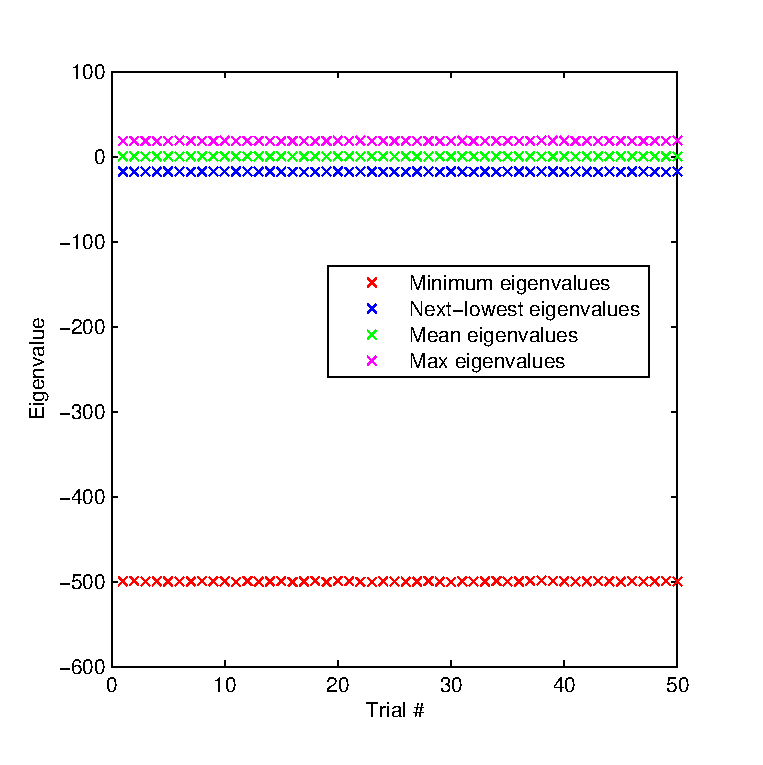
\includegraphics{p1}
\\
There is a clear separation of about 500 between the lowest and next-lowest eigenvalues.

\section{Problem 2}
We construct the Lorentz force law using quantum mechanical operators and Ehrenfest's theorem 
$\frac{d<\bv{L}>}{dt}=<\frac{\partial \bv{L}}{\partial t} >+\frac{i}{\hbar}<[\bv{H}, \bv{L} ]>$ for some operator L.
Our Hamiltonian is $H=\frac{1}{2m}\Pi^2+q\Phi$, with $\Pi = m\bv{v}=p-\frac{q}{c}A$.
\\
We want to find the force $\frac{d<m\bv{v}>}{dt}$. From Ehrenfest's theorem:
\begin{gather}
 \frac{d<m\bv{v}>}{dt}=<\frac{\partial m\bv{v}}{\partial t} >+\frac{i}{\hbar}<[\bv{H}, m\bv{v} ]>\\
 \frac{d<m\bv{v}>}{dt}=<\frac{\partial \Pi}{\partial t} >+\frac{i}{\hbar}<[\frac{1}{2m}\Pi^2+q\Phi, \Pi ]>
\end{gather}
The first term is:
\begin{gather}
 \frac{\partial \Pi}{\partial t}=-\frac{q}{c}\frac{\partial A}{\partial t}
\end{gather}
We now open up the commutator:
\begin{gather}
 [\frac{1}{2m}\Pi^2+q\Phi, \Pi ]= \frac{1}{2m}[\Pi^2, \Pi] + [q\Phi, \Pi]
\end{gather}
We evaluate the second commutator:
\begin{gather}
 [q\Phi, \Pi]=[q\Phi,p]+[q\Phi,-\frac{q}{c}A]\\
 [q\Phi, \Pi]=q(\Phi p-p\Phi)+0\\
 [q\Phi, \Pi]=-i\hbar q(-\nabla \Phi)\\
 [q\Phi, \Pi]=-\frac{q \hbar}{i}\nabla\Phi
\end{gather}
We now must evaluate $[\Pi^2, \Pi]$.
\begin{gather}
 [\Pi^2,\Pi] = [\Pi, \Pi]\Pi+\Pi[\Pi, \Pi]\\
 [\Pi, \Pi] = \sum_{m,n = i,j,k} [\Pi_m, \Pi_n]\\
 [\Pi_m, \Pi_n] = [p_m-\frac{q}{c}A_m,p_n-\frac{q}{c}A_n]\\
 [\Pi_m, \Pi_n]-\frac{q}{c}\frac{\hbar}{i}(-\frac{\partial A_m}{\partial n})-\frac{q}{c}\frac{\hbar}{i}(\frac{\partial A_n}{\partial m})
      =-\frac{q}{c}\frac{\hbar}{i}(\frac{\partial A_n}{\partial m}-\frac{\partial A_m}{\partial n} )
\end{gather}
This is just the curl of A, which is also the magnetic field B. 
Incorporating the $\frac{1}{2m}$ term, and substituting $\frac{\Pi}{m}=v$, we find:
\begin{gather}
  \frac{1}{2m}[\Pi^2,\Pi]=\frac{q}{2c}\frac{\hbar}{i}(v \times B - B \times v)
\end{gather}
We can now have all the terms in $\frac{d<m\bv{v}>}{dt}$,
\begin{gather}
 \frac{d<m\bv{v}>}{dt}=<-\frac{q}{c}\frac{\partial A}{\partial t}>+<\frac{i}{\hbar}\left( 
	-\frac{q \hbar}{i}\nabla\Phi+\frac{q}{2c}\frac{\hbar}{i}(v \times B - B \times v)   \right)>\\
 \frac{d<m\bv{v}>}{dt}=q(<-\nabla\Phi-\frac{1}{c}\frac{\partial A}{\partial t}+\frac{1}{2c}(v \times B - B \times v) >)	
\end{gather}
But $-\nabla\Phi-\frac{1}{c}\frac{\partial A}{\partial t}$ is the electric field E. 
So we have the Lorenta force law:
\begin{gather}
 \frac{d<m\bv{v}>}{dt}=q(<E-\frac{1}{2c}(v \times B - B \times v) >	
\end{gather}
For classical vectors $v\times B = -B \times v$, and this reduces to the classical Lorentz force law.


\section{Problem 3}
a) The Hamiltonian for a hydrogen atom in a electromagnetic field is:
\begin{gather}
 H=\frac{p^2}{2m}-e\Phi-\frac{e^2}{r}
\end{gather}
We then substitute $\Pi$ for p.
\begin{gather}
 H=\frac{1}{2m}\left(p-\frac{q}{c}A \right)^2-e\Phi-\frac{e^2}{r}
\end{gather}
\\
b) Expanding the kinetic energy term and truncating the $\frac{A^2}{c^2}$ term:
\begin{gather}
 H=\frac{p^2}{2m}-e\Phi-\frac{e^2}{r}-\frac{q}{2mc}\left(p\cdot A+A\cdot p \right)\\
 H_0 = \frac{p^2}{2m}-e\Phi-\frac{e^2}{r}\\
 H_1=-\frac{q}{2mc}\left(p\cdot A+A\cdot p \right)
\end{gather}
We choose the Coulomb gauge, so $\Phi=0$ and $\nabla \cdot \bv{A}=0$.
we can then write the pertrubing Hamiltonian as:
\begin{gather}
 H_1=-\frac{q}{mc}\left(p\cdot A\right)
\end{gather}
The vector potential $\bv{A}$ expressed in terms of creation/annihilation operators is:
\begin{gather}
 \sum_{k,\sigma}\frac{\sqrt{2\pi\hbar c^2}}{\omega}\left(a_{k,\sigma}e^{i(kx-\omega t)}
      +a_{k,\sigma}^{\dagger} e^{-i(kx-\omega t)} \right)
\end{gather}
\\
c) We now calculate the matrix elements of the perturbing Hamiltonian.
The states are direct products of the electronic state with the electromagnetic field state. 
The initial state has no photons, the final state has a single photon in the ``appropriate mode`` $\sigma',k'$.
The creation operator $a_{\sigma ', k'}$ creates a photon in the appropriate mode, so the matrix element $\braket{1_{\sigma',k'}|A|0}$ is just $e^{i\omega t}\frac{q\sqrt{2\pi\hbar}}{m \omega}$.

d) We write down the expression for the general matrix element, pull out the constants, and ignore the part of the vector potential with the annihilation operator since the initial state always has 0 photons.
\begin{gather}
 H_{(n'\ell 'm'),(n\ell m)}=\bra{1}\bra{n'\ell 'm'}\frac{q}{mc}\left(p\cdot A\right)\ket{n\ell m}\ket{0}\\
 H_{(n'\ell 'm'),(n\ell m)}= e^{i\omega t}\frac{q\sqrt{2\pi\hbar}}{m \omega}\bra{1}\bra{n'\ell 'm'}pe^{-ikx}a^{\dagger}\ket{n\ell m}\ket{0}
\end{gather}
The creation operator $a^{\dagger}$ will act on the electromagnetic part of the state to create a photon.
We take the Taylor series expansion of $e^{-ikx}$ and keep only the leading term (1). 
We can now focus on the electronic states:
\begin{gather}
 H_{(n'\ell 'm'),(n\ell m)}= \frac{q\sqrt{2\pi\hbar}}{m \omega}\bra{n'\ell 'm'}p\ket{n\ell m}
\end{gather}
The operator p is $\frac{\hbar}{i}\nabla$, but we look for a way to avoid doing a bunch of calculus.
We instead look at the commutation relations of the unperturbed Hamiltonian.
\begin{gather}
 H_0 = \frac{p^2}{2m}-\frac{e^2}{r}\\
 [H_0,x] = [\frac{p^2}{2m}-\frac{e^2}{r}, x] = [\frac{p^2}{2m}, x]+0\\
 [H_0,x] = \frac{1}{2m}\left[p[p,x]+[p,x]p \right]
\end{gather}
The commutator $[p,x]$ is $\frac{\hbar}{i}$, so we can write $p=\frac{im}{\hbar}[H_0,x]$.
We now have:
\begin{gather}
 H_{(n'\ell 'm'),(n\ell m)}=\frac{iq\sqrt{2\pi\hbar}}{\hbar \omega}\bra{n'\ell 'm'}[H_0,x]\ket{n\ell m}\\
 H_{(n'\ell 'm'),(n\ell m)}=\frac{iq\sqrt{2\pi\hbar}}{\hbar \omega}\bra{n'\ell 'm'}H_0x-xH_0\ket{n\ell m}\\
\end{gather}
This separates into two terms, one with $\bra{n'\ell 'm'}H_0x\ket{n\ell m}$ and one with $\bra{n \ell m}H_0^*x^*\ket{n'\ell ' m'}$.
But $H_0x\ket{n\ell m}=E_{n\ell m}\ket{n\ell m}$ and $H_0^*x^*\ket{n'\ell ' m'}=E_{n'\ell 'm'}\ket{n'\ell ' m'}$.
Since $\braket{n\ell m|n' \ell' m'}=\braket{n'\ell 'm'|n\ell m}$ we can write this as:
\begin{gather}
  H_{(n'\ell 'm'),(n\ell m)}=(E_{n\ell m}-E_{n'\ell 'm'})
	  \frac{iq\sqrt{2\pi\hbar}}{\hbar \omega}
	  \braket{n'\ell 'm'|n\ell m}
\end{gather}
The $\braket{n'\ell 'm'|n\ell m}$ integrals are solved by expaning one spherical harmonic in terms of the other, and are tabulated for small values of $n, \ell$ and $m$.
The seelction rules derived from the orthogonality of the spherical harmonics in the expansion will also prohibit transitions unles $|\ell'-\ell|=1$.
With a final state of $\ket{100}$ transitions from the $\ket{200}$ state is forbidden. The transition from the $\ket{211}$ state is allowed. 
The transition directly from the $\ket{322}$ state is also forbidden.

\end{document}
